
\section{Results} \label{sec:results}

% Total number of Java projects: 50 k (7.25\%)
% Total number of projects: 699331
% Total number of projects: 49 (0.1\%)

Around 50k Java projects were mined using the Boa infrastructure.
Of those projects, 49 are using \smu{} (representing 0.1\%).
This result is even less than the estimation made by Sandoz~\cite{psandoz14}.
An overview of the projects using \smu{} is presented in table~\ref{table:projects}

% latex table generated in R 3.1.2 by xtable 1.7-4 package
% Wed Feb  4 17:27:46 2015
\begin{table*}[htb]
\centering
\caption{Java Projects using \smu{}} 
\label{table:projects}
\begin{tabularx}{\textwidth}{|r|l|X|r|r|r|r|r|}
  \hline
\# & Name & Description & \# AST Nodes & \# Revisions & Lifetime & \# smU Calls & \# smU Literal \\ 
  \hline
1 & adtools & Amiga Development Tools (adtools) & 14911 k & 466 & 6 years & 421 &   0 \\ 
  2 & amino & Concurrent Building Block & 255 k & 691 & 4 years &  53 &   0 \\ 
  3 & amock & Java Mock libarary for static method & 13 k &   3 & 1 month &  14 &   0 \\ 
  4 & android & Android on PXA270 & 4836 k & 146 & 1 year &  77 &   0 \\ 
  5 & aojunit & An aspect-oriented extension to JUnit & 1 k &   5 & 1 day &   1 &   0 \\ 
  6 & archaiosjava & Scalable and fast libraries for Java & 11 k &  17 & 14 days & 102 &   0 \\ 
  7 & beanlib & Java Bean Library & 119 k & 854 & 6 years &   4 &   0 \\ 
  8 & caloriecount & Track what you eat & 352 k & 202 & 5 months &  10 &   0 \\ 
  9 & cegcc & CeGCC - Cross development for Pocket PC & 2203 k & 1449 & 4 years & 101 &   0 \\ 
  10 & cgnu & CGNU (Clean GNU) & 2135 k &  60 & 1 month & 101 &   0 \\ 
  11 & classreach & Identifies unused Java classes and methods & 196 k &  69 & 2 years &  10 &   0 \\ 
  12 & clipc & Library for IPC & 228 k & 278 & 6 months &  10 &   0 \\ 
  13 & concutest & Tools to test concurrent Java programs & 550 k &  14 & 2 years & 185 &   0 \\ 
  14 & ec & ec-gin Europe China Grid InterNetworking & 635 k &   9 & 2 months &  10 &   1 \\ 
  15 & essence & Essence Java Framework & 157 k & 293 & 2 years &  75 &   0 \\ 
  16 & essentialbudget & Essential Budget & 60 k &  55 & 4 months &  20 &   2 \\ 
  17 & glassbox & Troubleshooting and monitoring agent & 99 k & 458 & 4 years &   1 &   0 \\ 
  18 & grinder & Load testing framework & 770 k & 4334 & 11 years &   6 &   0 \\ 
  19 & high & Highly Scalable Java & 37 k &  78 & 2 years &  37 &   0 \\ 
  20 & hlv & Collection of high level view plugins for eclipse & 33 k & 278 & 1 year &   0 &   4 \\ 
  21 & ikvm & JVM for .NET Framework and Mono & 531 k & 3980 & 10 years & 123 &   0 \\ 
  22 & jadoth & abstraction utils and frameworks & 619 k & 2922 & 3 years & 949 &   0 \\ 
  23 & janetdev & Ja.NET - Java Development Tools for .NET & 10034 k & 366 & 2 years & 280 &   0 \\ 
  24 & janux & Java directly on the Linux Kernel & 564 k &  25 & 1 month &  10 &   0 \\ 
  25 & java & Lightweight Java Game Library & 571 k & 3841 & 10 years &   6 &   0 \\ 
  26 & javapathfinder & Verifies Java bytecode programs & 9952 k & 4038 & 6 years &   0 &   4 \\ 
  27 & javapayload & Payloads to be used for post-exploitation & 74 k &  92 & 2 years &  28 &   1 \\ 
  28 & jaxlib & Platform independent Java library & 5405 k & 3208 & 11 years &  42 &   3 \\ 
  29 & jigcell & Computational biology problem solving & 3573 k & 5286 & 8 years &   0 &   3 \\ 
  30 & jikesrvm & The Jikes Research Virtual Machine (RVM) & 9026 k & 16068 & 10 years &  32 &  16 \\ 
  31 & jnode & JNode: new Java Operating System & 44401 k & 11972 & 10 years & 2104 &   0 \\ 
  32 & jon & Java Object Notation & 29 k & 118 & 1 year &   3 &   0 \\ 
  33 & jprovocateur & RAD for Ajax applications in Java & 197 k & 934 & 2 years &  10 &   2 \\ 
  34 & junitrecorder & Record test cases & 34 k &  18 & 2 months &   1 &   0 \\ 
  35 & katta & Lucene in the cloud & 169 k & 478 & 1 year &  31 &   0 \\ 
  36 & l2next & L2 Private Server code & 39 k &  22 & 1 month &  26 &   0 \\ 
  37 & lockss & Lots of Copies Keep Stuff Safe & 11551 k & 23048 & 11 years &   0 &   2 \\ 
  38 & neurogrid & P2P Bookmark Organiser & 337 k & 738 & 5 years &   2 &   0 \\ 
  39 & osfree & osFree operating system & 119 k & 1124 & 5 years &  96 &   0 \\ 
  40 & ps2toolchain & Toolchain for the Playstation 2's & 4298 k &   8 & 1 day & 202 &   0 \\ 
  41 & simulaeco & Semester project & 136 k &  66 & 4 months &  10 &   2 \\ 
  42 & snarej & Snare's Not A Risc OS Emulator in Java & 111 k &  82 & 1 month &  19 &   0 \\ 
  43 & statewalker & Graph traversing library & 477 k & 432 & 3 years &  36 &   2 \\ 
  44 & takatuka & TakaTuka Java Virtual Machine & 1176 k & 2637 & 3 years & 107 &   0 \\ 
  45 & timelord & A tool for estimating and tracking time & 697 k & 546 & 2 years &  40 &   0 \\ 
  46 & ucl & A final year project by UCL students & 1639 k &  70 & 3 months &   0 &   1 \\ 
  47 & vcb & Component Based Development tool & 602 k & 2446 & 3 years &  11 &   0 \\ 
  48 & x10 & Experimental language for DARPA/HPCS & 12292 k & 25432 & 9 years & 279 &   0 \\ 
  49 & xbeedriver & Driver for the ZigBee network & 119 k &   6 & 3 days &  10 &   2 \\ 
   \hline
\end{tabularx}
\end{table*}



The figure~\ref{fig:usage} shows how many times a method is called. Grouped by functional group.

\begin{figure*}[htb]
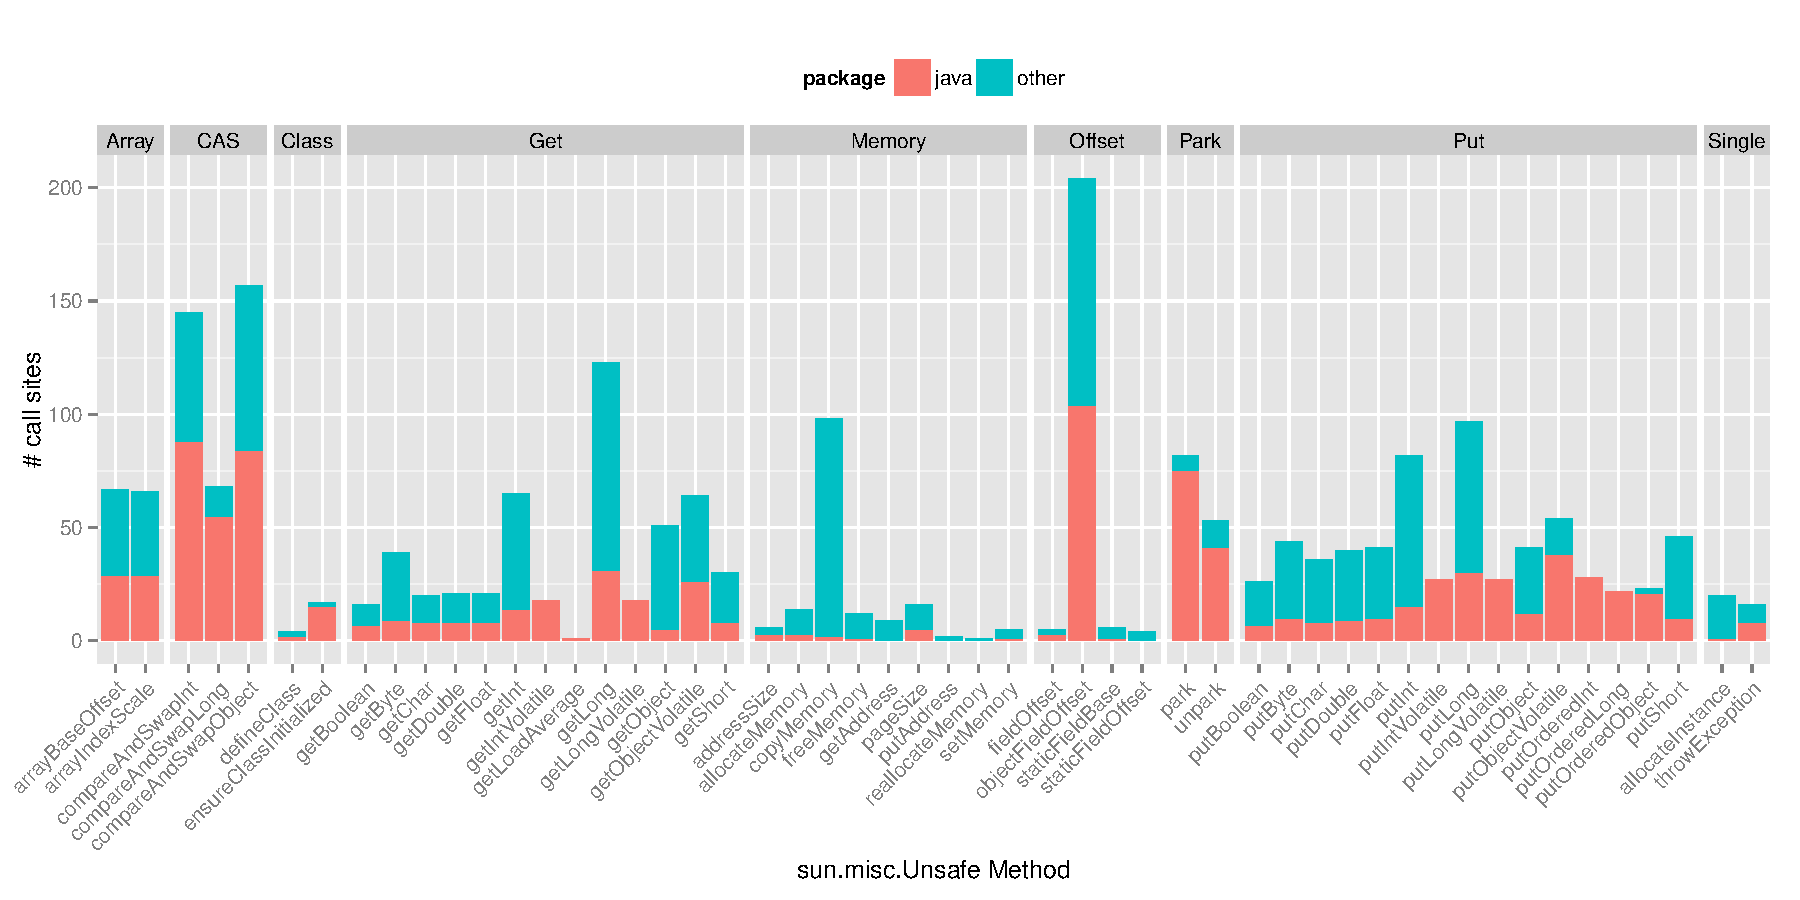
\includegraphics[width=\textwidth]{unsafe-plot-usage}
\caption{sun.misc.Unsafe methods usage} \label{fig:usage}
\end{figure*}

The most called is \texttt{objectFieldOffset}. Because the result is then used by many other calls to Unsafe.

\subsection{Stackoverflow}

Google search for sun.misc.unsafe site:stackoverflow.com
returns about 1,360 results.

Searching for the term: "unsafe java" on stackoverflow returns 1,241 results.
While searching for only the term "sun.misc.unsafe" returns 318 results.

Representative SO ids:



